\section{Viabilidade Financeira}

O projeto de análise de viabilidade financeira consiste em averiguar a garantia de lucro sobre as despesas do projeto. Portanto, nesse projeto será descrito cada processo a fim de fazer essa verificação.

\subsection{Gerenciamento de Custos}

Nesse tópico, serão abordados temas de investimento inicial e de desenvolvimento do projeto, incluindo tópicos de análise de requisitos, desenvolvimento, manutenções e imprevistos.

\subsubsection{Análise de Requisitos e Desenvolvimento}

Para iniciar o projeto, é necessário fazer os primeiros planejamentos, elicitação de requisitos, abstrair e concretizar as primeiras ideias e fazer os primeiros planejamentos (diagramas, cronogramas e documentação). Logo após, o projeto chega na fase de desenvolvimento, onde é começado a se tornar real.

Contudo, o projeto não vai possuir nenhum custo de análise e implementação do sistema, devido ao fato de ser um projeto educacional.

\subsubsection{Manutenções}

Inevitavelmente, manutenções do sistema ocorrerão pós finalização do projeto e estar devidamente funcional em produção. Contudo, os custos de manutenções também não serão cobrados, devido a ser um projeto educacional.

\subsection{Custos de deploy e de Ambiente de Produção}

Nesse tópico, são apresentados os custos de manter o sistema funcional e disponível para os usuários. Desse modo, será feito uma previsão anual de cada plataforma utilizada:

\subsubsection{Frontend} 

Tendo em vista que o projeto é \textit{mobile} voltado para dispositivos Android, será publicado na PlayStore, estimando um valor de 25.00 USD anual. 

\subsubsection{Backend}

Inicialmente gratuíto no Amazon EC2, sendo permitido 750h de instâncias por mês durante o período de 12 meses.

A partir do momento que for necessário grande porte, será indicado o plano Sob Demanda do Amazon EC2, que garante viabilidade econômica e estratégica (visto que o preço é calculado a partir do uso). 

Nesse plano, o custo de transferência de dados (ou seja, entrada e saída de dados) geram o valor de, na região de São Paulo, no máximo 0,15 USD por GB.

Na \autoref{fig:prices-ec2}, seguem os preços dos planos Sob Demanda na região de São Paulo para Linux usando tipo de instância geral com 1 vCPU.

\begin{figure}[h]
  \centering
  \caption{Preços do Amazon EC2 - Sob Demanda \\ \cite{AmazonEC2}}
  \label{fig:prices-ec2}
  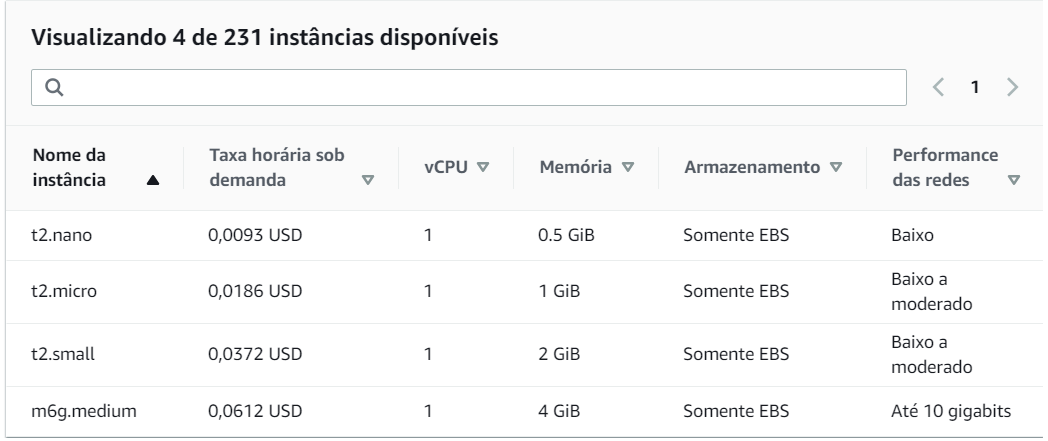
\includegraphics[scale=0.6]{prices-ec2}
\end{figure}

\subsubsection{Banco de Dados} 

Inicialmente gratuíto no Amazon RDS, sendo permitido 750h de instâncias durante o período de 12 meses. O Amazon RDS possui suporte a vários Sistemas Gerenciadores de Banco de Dados (SGBD), incluindo o MySQL, que foi o SBGD optado para desenvolver a aplicação Lixt.

A partir do momento que for necessário grande porte, será indicado o plano Sob Demanda do Amazon RDS, que garante viabilidade econômica e estratégica (visto que o preço é calculado a partir do uso).

Na \autoref{fig:prices-rds}, seguem os preços dos planos Sob Demanda na região do Leste dos EUA (única opção disponível em 07/06/2021).

\begin{figure}[h]
  \centering
  \caption{Preços do Amazon RDS - Sob Demanda \\ \cite{AmazonRDS}}
  \label{fig:prices-rds}
  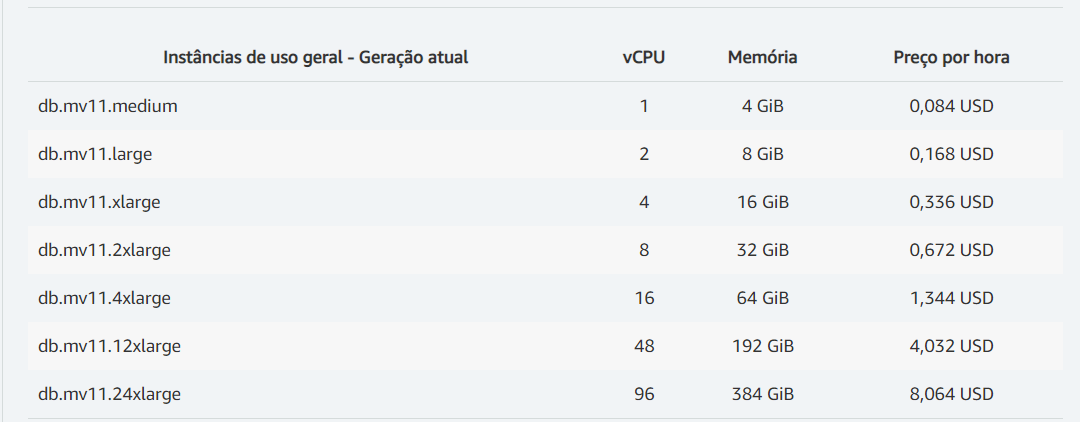
\includegraphics[scale=0.6]{prices-rds}
\end{figure}	

\subsection{Medidas de Obtenção de Retorno Financeiro}

Para gerar uma receita positiva a fim de obter lucro, haverá duas formas principais de retorno financeiro:
\begin{itemize}
	\item \underline{Cobrança do aplicativo}: O aplicativo estará disponível gratuitamente na PlayStore, não gerando, portanto, retorno financeiro.
	\item \underline{Propaganda/Recomendação}: Será utilizado mediador de anuncio AdMob (responsável por conectar aplicações e anunciantes), onde o valor varia por visualizações de anúncios e cliques neles. Contudo, no próprio site do admob, é citado um caso no qual houve 300.000 downloads e recebia, através do AdMob, 100 USD por dia. \cite{GoogleAdMob}
\end{itemize}
